\documentclass[10pt,a4paper]{article}
\usepackage[utf8]{inputenc}
\usepackage{amsmath}
\usepackage{amsfonts}
\usepackage{mathtools}
\usepackage{amssymb}
\usepackage{graphicx}
\usepackage{subcaption}
\usepackage{dsfont}
\usepackage[strict]{changepage}
\usepackage{float}
\usepackage{parskip}
\makeatletter
\newcommand*{\transpose}{%
  {\mathpalette\@transpose{}}%
}
\newcommand*{\@transpose}[2]{%
  % #1: math style
  % #2: unused
  \raisebox{\depth}{$\m@th#1\intercal$}%
}

\author{Adam Jalkemo \texttt{adam@jalkemo.se} \and
Alexander Israelsson \texttt{israelsson.alexander@gmail.com} \and
Emil Westenius \texttt{emil@westenius.se} \and
Jonathan Andersson \texttt{mat11ja1@student.lu.se}}
\title{Adaptive Friction Compensation}
\begin{document}
\maketitle
\section{Introduction}
In this project a Furuta pendulum process will be used. The pendulum will be stabilized in the inverted position using a swing up controller and a top controller. When controlling the pendulum in the top position limit cycles will occur due to friction. By compensating for the friction we aim to stabilize the pendulum, the friction will be estimated using an adaptive method. To do this a Java controller and interface will be implemented and run on a linux computer.
\section{Theory}
\begin{itemize}
\item Explain which theory is interesting and what is difficult, what is the focus of the project? I.e. Friction estimation and compensation, explain RLS and other estimation tools, explain how the compensation is done. 
\item What can be written about real time part?
\end{itemize}
\subsection{Friction estimation}
\begin{itemize}
\item RLS
\item Chosen regressor and chosen equation
\item top position/bottom position
\item in top position, when and why do we turn off estimation
\item Aternatives to RLS
\end{itemize}
\subsection{Compensation}
just straight adding friction? other way?
in top position, when and why do we turn off compensation
\subsection{Real-time implementation}
\section{Program Structure}
For our suggested solution we will need one thread for the GUI and one for the controller. To communicate with the Furuta process we will use the analog box normally used during the control labs at LTH. The realtime package from Automatic Control at LTH will be used for communication in the GUI and controller implementation. It will be important to synchronize the controller calculations with the user inputs. A general overview can be seen in figure \ref{fig:uml}.
\begin{figure}[H]
\centerline{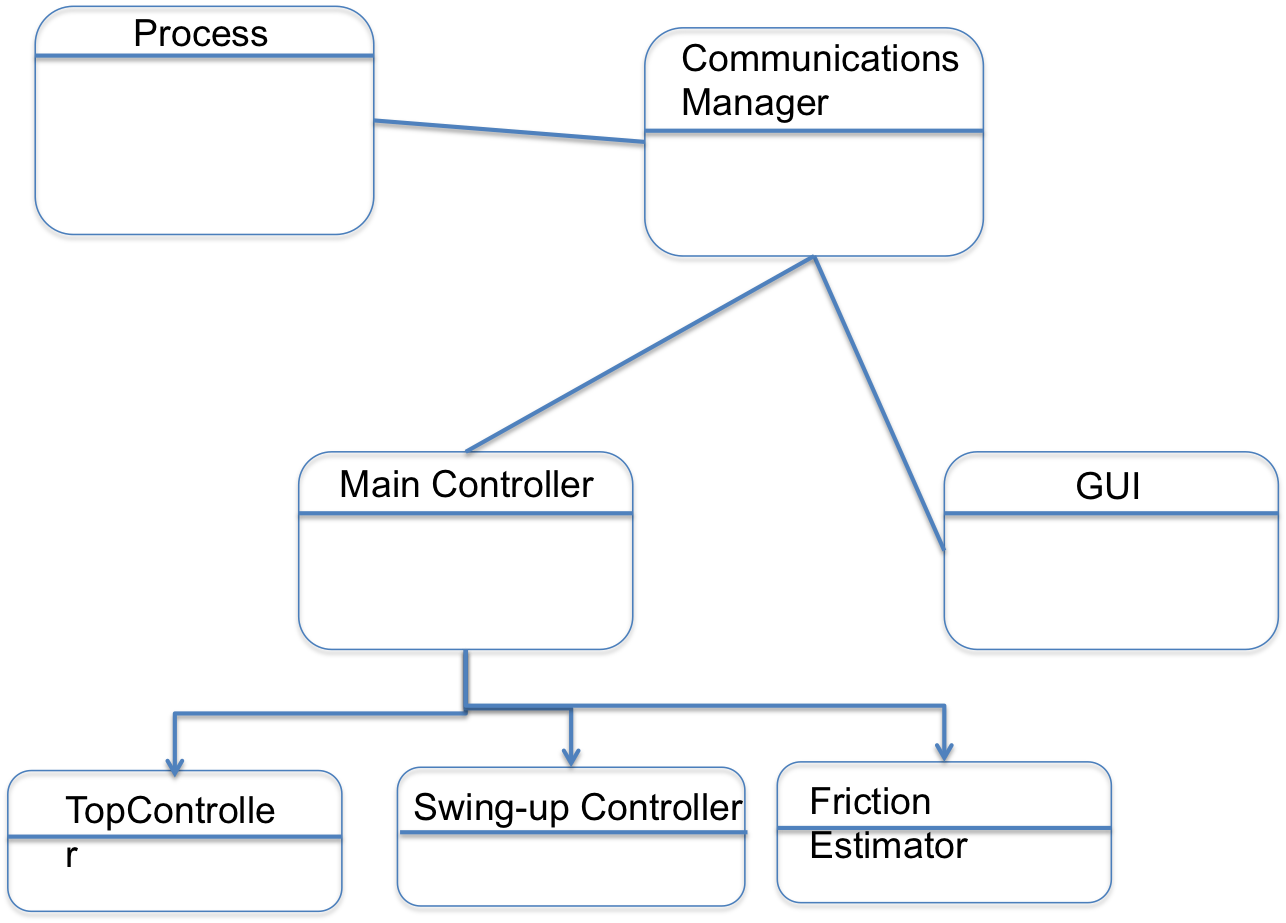
\includegraphics[scale=0.7]{umlfuruta.png}}
\caption{Overview of the program structure}
\label{fig:uml}
\end{figure}
\subsection{GUI}
The operator should be able to change controller parameters for both types of controller, the top controller and the swing up controller, as well as change the parameters for the friction estimation. 

The GUI will plot the outputs from the Furuta pendulum, the friction estimation, control signal, both uncompensated as well as the compensated signal. We aim to have different regressor modes for the friction compensation and the operator can therefore change different parameters depending on the regressor chosen. 

We aim to be able to change all parameters on-line.
\subsection{Controller}
For the swing up a Lyapunov based controller will be used. In the top position a LQG controller will be used. The controllers will be implemented in Java.
Models for Coulomb and viscous friction and additional models for asymmetric friction will be considered. The friction will be estimated using RLS. The regression model will depend on which friction model we choose to consider. 
\subsubsection{Swing-up}
\begin{itemize}
\item Lyaponov
\item Catching area
\end{itemize}
\subsubsection{Top Controller}

\section{Results}
\begin{itemize}
\item Different equations for RLS gives different friction estimations
\item Different P results
\item other estimation tools? differences?
\item 
\end{itemize}
\section{Discussion}
\section{Conclusions}










\section{Program structure}

%% MORe STUFFS??

%ToDo UML AND DESCRIPTION OF CLASSES AND PACKAGES



%Todo what parameters can be changed.

\subsection{Controller}


\subsection{GUI}


\section{Time plan}
\begin{table}[H]
\centering
\caption{Time plan}
\label{hoho}
\begin{tabular}{|l|l|l|}
\hline
Week & Description & Main Responsibility \\ \hline
13 & Hand in project plan & All members \\ \hline
& Begin GUI implementation & Adam \\ \hline
& Begin implementation of Java controller & Alexander \\ \hline
& Begin implementation of Matlab controller & Jonathan \\ \hline
& Research on friction estimator and model & Jonathan \\ \hline
14 & Working GUI implementation & Adam \\ \hline
& Write skeleton for report & Emil \\ \hline
& Working basic implementation of Java controller & Alexander \\ \hline
& Working basic implementation of Matlab controller & Jonathan \\ \hline
15 & Finished Matlab controller for tests & Jonathan \\ \hline
& Predictive theory complete  & Emil \\ \hline
& All code complete, begin testing and tuning & All members \\ \hline
16 & Begin Predictive presentation & Alexander \\ \hline
& Realtime theory complete & Adam \\ \hline
17 & Predictive presentation 29/4 & \\ \hline
18 & Adapt presentation for Realtime course & Jonathan \\ \hline
19 & Fine tune until perfection & All Members \\ \hline
20 & Realtime presentation 19/5  & \\ \hline
\end{tabular}
\end{table}
The aim is to finish the GUI as soon as possible to be able to properly evaluate our controller. The controller will first be done in Matlab since a working solution already exist except for the RLS estimator. This also makes it easier to evaluate the controller in Java since the expected behavior is then known.

The report will be written concurrently to the work on the other parts.




\section{Responsibilities}
\begin{itemize}
\item Theory - Emil
\item Report - Emil
%	What estimators to use\\
%	What friction model
\item Friction controller in MATLAB - Jonathan
\item Controller in Java - Alexander
%	Friction\\
%	Swingup\\
%	Top controller
\item GUI - Adam
\item Presentation - Jonathan

\end{itemize}
\begin{itemize}
\item Write brake function for arm movement
\item Write stabilization function in bottom position
\item omega0 estimation function
\item Implement friction estimation for top position
\item (implement lower position friction estimation
\item Save parameters to harddrive
\item Start looking at predictive 



\end{itemize}

\end{document}

